\section{Implementation}
\label{sec:alg}
We implemented our tool as an extension to a GHC Haskell add-on, called
Quelea 
\cite{quelea},
previously developed by Sivaramakrishnan and two of the authors of this paper.
Quelea maintains a causally consistent cache on top of Cassandra, and \emph{all} operations whose contract is satisfied under causal
consistency, are performed witnessing that cache (even if they require considerably
weaker guarantees than causal).

In \tool, we maintain a generic cache equipped with a tagging mechanism,
where each operation is associated with a tag, and is allowed to witnesses only the subset of effects in the
cache, holding that tag (i.e. effects that are in the \emph{logical
cache} associated with that operation). We implemented a dependency finder mechanism in
\tool, that is used to verify the presence of arbitrarily defined dependencies of an
effect in each logical cache. Consequently, \tool's filtration and blocking
mechanisms are added to the runtime system, which rely on this dependency finder to keep each logical cache
consistent according to its associated contract. Specifically, 
considering a dependency relation $R$ and a replica containing a localset $V$
of effects, an effect $\eta$ is allowed to enter a logical cache, only if
$\trunc{R}_V^{-1}(\eta)$ is already in that cache. 


%the memoization technique
Considering the arbitrary length of the dependency relations expressible
in our contract language, and the fact that verifying the presence of
dependancies for an effect might fail for an unbounded number of trials
until all the dependencies arrive, we noticed considerable redundencies
in our dependency finder mechanism, which adversely affected the
performance.
To overcome this problem, we implemented a simple memoization technique in \tool\
that extends the binary notion of dependency presence to the
\emph{degree of dependency presence} (\DDP{}) representing 
the maximum \emph{depth} (or size) of the dependencies of an effect, whose presence have been
verified so far. 
Consequently, when verification of the presence of
dependencies for an effect fails, the runtime system can avoid redundant
computations the time it tries to verify the same property for the
same effect.
\tool's runtime, by performing
periodic \DDP{} refreshes, tries to assign larger \DDP{} values to each effect
when more dependencies arrive at the replica. We leave the details of
this technique, captured as an operational semantics in 
appendix \ref{appendix:large_semantics} for an interested reader.








\begin{comment}
%intro
While the semantics defines \emph{what} \emph{what} subset of
effects at a replica  must be witnessed by every operation, it does
not address \emph{how} to realize efficient construction of that subset.

%how cache works
\tool maintains a consistent cache on top of each replica by periodically
reading from the underlying ECDS, where an effect $\eta$ is moved to the
cache only if the cache already includes {\footnotesize
$\trunc{R}_V^{-1}(\eta)$}. Consequently, all operations under \UB{}
contracts can be immediately executed
by witnessing the cache, which is a closed subset (not necessarily maximal) 
of $V$, the set of effects present at the replica. 
Moreover, \LB{} contracts can also be satisfied, by blocking  operations 
until effects of all previous operations from the same session enter
the cache, in which case the current operation can proceed and witness \emph{all}
effects present at the replica.

%the memoization technique
Additionally, we implemented a simple memoization technique in \tool\
that extends the binary notion of dependency presence to the
\emph{degree of dependency presence} (\DDP{}) representing 
the maximum \emph{depth} (or size) of the dependencies of an effect, whose presence have been
verified so far. 
Consequently, when verification of the presence of
dependencies for an effect fails, the runtime system can avoid redundant
computations the time it tries to verify the same property for the
same effect.
\tool's runtime, by performing
periodic \DDP{} refreshes, tries to assign larger \DDP{} values to each effect
when more dependencies arrive at the replica. 
Specifically, at each refresh, the \DDP{} of an effect $\eff$ is increased from $i$ to $i+1$ if
all effects in $r_{i+1}^{-1}(\eff)$ already have \DDP{} values at least
equal to $i$.

% example
%%%SJ: This is confusing - you need to give an example of a
%%%redundant computation, otherwise this paragraph will not be understood by the reader
For example, consider a contract with dependency relation
$\Rel=\soZ;\visZ;\soZ$, and a newly arrived effect $\eta$ to the
replica, whose \DDP{} is initially set to 0. 
During the next refresh, $\eta$ is given the value 1, if all
effects in $\soZ^{-1}(\eta)$ have \DDP{} equal to 0 (i.e. are present at the
replica). Similarly, $\eta$ is given the value 2, if all effects in
$\visZ^{-1}(\eta)$ have \DDP{} value of at least 1, which means that 
$(\soZ;\visZ)^{-1}_V(\eta)$ is now present at the replica and
consequently, $\eta$ can
be safely added to the consistent cache (Fig.\ref{fig:avail_deg}).
Using this technique, \tool avoid redundant computations of potentially large
dependency relations.
%\begin{figure}[t]
	\centering
	\setlength{\fboxsep}{6pt}%
	%\framebox[0.87\textwidth]{
	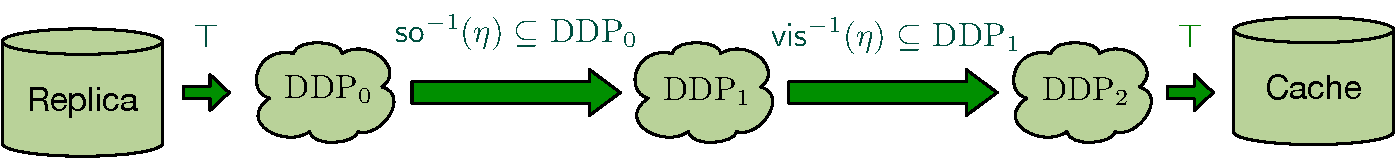
\includegraphics[scale =
	0.4]{Figures/Availability_deg.pdf}
	%}
	\\ 
	\hrulefill
\caption{Example of stepwise progress of effects before entering the
cache}
\label{fig:avail_deg}
\end{figure}

\end{comment}
